
	\begin{definition} 
		\emph{Аффинная алгебра}~--- это координатное кольцо некотрого аффинного многообразия. 
	\end{definition}

	\begin{remark}
		Как мы увидим немного позже, эквивалентно можно говорить, что аффинная алгебра~--- это конечнопорожденная редуцированная алгебра. 
	\end{remark}

	\begin{theorem}\label{ht(p) + dim(B/p)} \hypertarget{bilet_15}{}
		Пусть $B$~--- целостная аффинная алгебра над $\Bbbk$ (или, что эквивалентно, конечно-порожденная целостная $\Bbbk$-алгебра), а $\fp \in \Spec{B}$. Тогда 
		\[
			\Ht{\fp} + \dim{B/\fp} = \dim{B}.
		\]
	\end{theorem}
	\begin{proof}
		Будем вести индукцию по $\dim{B}$. База ($\dim{B} = 0$) очевидна. 

		\RNum{1.} Пусть $B = \Bbbk[x_1, \ldots, x_n], \ \dim{B} = n$. Возьмём $\fp \in \Spec{B}$, $\Ht{\fp} = m$, то есть 
		\[
			0 \subset \fp_1 \subset \fp_2 \subset \ldots \subset \fp_m = \fp.
		\]
		Тогда $\Ht{\fp_1} = 1$, но тогда идеал $\fp_1$~--- главный, т.е. $\fp_1 = (q)$. В самом деле, иначе мы можем взять образующую, разложить её на неприводимые множители (кольцо многочленов факториально) и взять неприводимымй сомножитель, попадающий в $\fp_1$. Так мы получим простой идеал, меньший $\fp_1$ и придём к противоречию. 

		Рассмотрим тогда $\fp/(q) \lei B/(q)$, $\fp/(q) \in \Spec{B/(q)}$. Так как $\dim{A/(q)} = \dim{B} - 1$, мы можем применить индукционное предположение: 
		\[
			\Ht{\fp/(q)} + \dim{B/\fp} = \dim{B} - 1. 
		\]

		Докажем, что $\Ht{\fp/(q)} = \Ht{\fp} - 1$. Очевидно, что $\Ht{\fp/(q)} \ge \Ht{\fp} - 1$. С другой стороны, если $\varphi\colon B \to B/(q)$, то если есть цепочка 
		\[
			0 \subset \fq_1 \subset \ldots \subset \fq_{s} = \fp/(q),
		\]
		то есть и цепочка для $\fp$:
		\[
			0 \subset (\fq) \subset \varphi^{-1}(0) \subset \varphi^{-1}(\fq_{1}) \subset \ldots \subset \varphi^{-1}(\fq_{s}) = \fp.
		\]
		\RNum{2.} Пусть $B$~--- произвольная конечнопорожденная целостная $\Bbbk$-алгебра. Вспомним теорему о спуске: 

		\begin{theorem}[О спуске] 
			Пусть $A \subset B$~--- целостные и $B/A$~--- цело. Пусть $\fq_{m} \in \Spec{B}, \ \fp_m \in \Spec{A}$~--- простые. Тогда для любой цепочки простых идеалов
			\[
				\fp_0 \subset \fp_1 \subset \ldots \subset \fp_m \subset A
			\]
			существует цепочка простых идеалов 
			\[
				\fq_0 \subset \fq_1 \subset \ldots \subset \fq_m \subset B\colon \fq_i \cap A = \fp_i.
			\]
		\end{theorem}

		Так вот, по лемме Нётер о нормализации $B$~--- целое расширение $A = \Bbbk[x_1, \ldots, x_n]$, $\dim{B} = \dim{A}$. Тогда по теореме о спуске для $\fq \in \Spec{B}$ мы имеем $\Ht{\fq} \ge \Ht{\fq \cap A}$. Кроме того, расширение 
		\[
			A/\fq \cap A \hookrightarrow B/\fq
		\]
		тоже целое, откуда $\dim{A/\fq \cap A} = \dim{B/\fq}$.  Тогда мы имеем 
		\[
			\dim{B/\fq} + \Ht{\fq} \ge \Ht\lr*{\fq \cap A} + \dim\lr*{A/\fq \cap A}
		\]
		По пункту $\RNum{1}$, правая часть равна $\dim{A} = \dim{B}$, то есть мы показали, что 
		\[
			\dim{B/\fq} + \Ht{\fq} \ge \dim{B}.
		\]
		Но, неравенство в другую сторону очевидно.

	\end{proof}

	\begin{corollary}
		Пусть $B$~--- целостная конечно-порожденная алгебра, $f \in B, \ f \neq 0$ и $f$ необратим. Пусть $\fp$~--- минимальный простой идеал, содержащий $f$. Тогда 
		\[
			\dim{B/\fp} = \dim{B} - 1.
		\]
	\end{corollary}
	\begin{proof}
		По теореме~\ref{ht(p) + dim(B/p)} мы имеем 
		\[
			\Ht{\fp} + \dim{B/\fp} = \dim{B}.
		\]
		Но, по теореме Крулля о главных идеалах (hauptidealsatz), $\Ht{\fp} = 1$, откуда мы имеем нужное.  
	\end{proof}

	Переформулируем это на алгебро-геометрический язык: 

	\begin{corollary}
		Пересечение неприводимого многообразия $X$ с гиперповерхностью или пусто, или имеет размерность хотя бы $\dim{X} \ge 1$. 
	\end{corollary}

	Отсюда получаем вот такое следствие: 
	

	\begin{statement}\label{dim{X} - m} 
		Все неприводимые компоненты $Z(I(X) + (f_1, \ldots, f_m))$ имеют размерность хотя бы $\dim{X} - m$.		
	\end{statement}
	
	\begin{corollary}\hypertarget{bilet_16}{}
		Пусть $f_1, \ldots, f_m \in \Bbbk[x_1, \ldots, x_n], \ m < n$ и $f_1(0) = \ldots = f_m(0) = 0$. Тогда система 
		\[
			\begin{cases} 
			f_1 = 0 \\ 
			\vdots \\
			f_m = 0
			\end{cases}
		\]
		имеет ненулевое решение. 
	\end{corollary}
	\textcolor{red}{Вот про это следствие еще надо всё понять.}

	

	\subsection{Регулярные функции}

	\begin{definition} 
		Будем говорить, что $X$~--- \emph{квазиаффинное многообразие}, если $X$~--- открытое подмножество аффинного многообразия. 
	\end{definition}

	\hypertarget{bilet_4}{}

	\begin{definition} 
		Пусть $X \subset \AA^{n}_{\bk}$~--- квазиаффинное. Будем говорить, что отображение $f\colon X \to \Bbbk$~--- регулярное в точке $p$, если существует окрестность $U \ni p$ и многочлены $g, h \in A = \bk[x_1, \ldots, x_n]$ такие, что 

		\begin{itemize}
			\item $h$ не имеет нулей в $U$,
			\item $f\vert_{U} = g/h$.
		\end{itemize}
		
		Функция $f$ называется \emph{регулярной} на $X$, если она регулярна в каждой точке $X$. 
	\end{definition}


	Регулярные функции на $X$ образуют кольцо, которое мы будем обозначать $\cO(X)$. 

	\begin{remark}
		Например, все многочлены~--- регулярные функции на $\AA^n$. 
	\end{remark}

	\begin{theorem}\label{O(X) = A(X)} 
		Пусть $X$~--- аффинное многообразие. Тогда 
		\[
			\cO(X) \cong A(X) = \Bbbk[x_1, \ldots, x_n]/I(X).
		\]
	\end{theorem}
	\begin{proof}
		Сначала отметим, что каждый многочлен очевидно определяет регулярную функцию на $\AA^n$, а значит и на $X$. Так мы строим гомоморфизм 
		\[
			\alpha\colon \Bbbk[x_1, \ldots, x_n] \to \cO(X), \quad f \mapsto f.
		\]
		Но, его ядро~--- это в точности $I(X)$: 
		\[
			\Ker{\alpha} = \{ f \in \bk[x_1, \ldots, x_n]\colon f\vert_{X} = 0 \} = I(X).
		\]
		Значит, у нас есть инъективный гомоморфизм $A(X) \hookrightarrow \cO(X)$. Покажем, что он сюръективен. 

		 Рассмотрим $f \in \cO(X)$. По определению, у любой точки $x \in X$ существует окрестность $U_x$ и многочлены $p_x, q_x$ такие, что $q_x f = p_x$ в $U_x$, причём $q_x$ не обращается в 0 на $U_x$. Так как $X \setminus U_x$ замкнуто, $X \setminus U_x = Z(\fa)$ для некоторого идеала $\fa$ и легко видеть, что 
		 \[
		 	Z(\fa) \subset X = Z(I(X)) \implies I(X) \subset \fa.
		 \]
		 Тогда, если мы возьмём $s \in \fa \setminus I(X)$, мы получим, что
		 \[
		 	s \cdot q_x \cdot f = s \cdot p_x \quad \text{ на всём } X, \text{ так как }
		 \]
		 \begin{itemize}
		 	\item $s \in Z(\fa) = X \setminus U_x$, что значит, что $s\vert_{X \setminus U_x} = 0$ и и на $X \setminus U_x$ это равенство превращается в $0 = 0$.

		 	\item А на $U_x$ это равенство получается домножением $q_x f = p_x$ на $s$.
		 \end{itemize}

		 Причём, выберем $s$ так, чтоб $s(x) \neq 0$. Мы можем так сделать, так как если нет, то 
		 \[
		 	\begin{cases} \forall s \in \fa \setminus I(X) \quad s(x) = 0 \\ \forall s \in I(X) \quad s(x) = 0 \end{cases} \implies \forall s \in \fa \quad s(x) = 0,
		 \]
		 но тогда $x \in Z(\fa) = X \setminus U_x$ (что абсурдно). 
		 
		 Итак, выбрав такой $s$ мы построили для любой точки $x$ многочлены $p_x'$ и $q_x'$ такие, что 
		 \[
		 	\forall y \in X \quad q_{x}'(y) f(y) = p_x'(y)  \text{ и } q'_x(x) \neq 0.
		 \]
 
		 Теперь рассмотрим идеал $\sum_{x \in X} (q_x') + I(X)$ в кольце $\bk[x_1, \ldots, x_n]$ и покажем, что он совпадает со всем кольцом. Предположим противное, тогда он содержится в некотором максимальном идеале $\fm \in \Spec(\bk[x_1, \ldots, x_n])$. Но тогда 
		 \[
		  	Z\lr*{\sum_{x \in X} q_x' + I(X)} \supset Z(\fm) = \mathrm{pt} \in \AA^n \implies \forall x \in X \ q'_x(\mathrm{pt}) = 0, \quad \forall h \in I(X) \ h(\mathrm{pt}) = 0.
		  \] 
		  Это даёт провтиворечие, так как 
		  \begin{itemize}
		  	\item Если $\mathrm{pt} \notin X$, то не может быть такого, что $\forall h \in I(X) \ h(\mathrm{pt}) = 0$. 

		  	\item Если же $\mathrm{pt} \in X$, то по построению $q'_{\mathrm{pt}}(\mathrm{pt}) \neq 0$.
		  \end{itemize}

		 	Итак, мы показали, что 
		 	\[
		 		\sum_{x \in X} (q_x') + I(X) = (1) \implies \sum_{x \in X} (\overline{q_x'}) = (\overline{1}) \text{ в } A(X),
		 	\]
		 	откуда сушествуют $\overline{\ell_{x_i}} \in A(X)$ такие, что 
		 	\[
		 		\sum_{i = 1}^{N} \overline{\ell_{x_i}} \cdot \overline{q'_{x_i}} = \overline{1} \quad \text{ на } X.
		 	\]
		 	Но, ранее мы показали, что $q_{x}' \overline{f} = p_x'$ на $X$, то, домножая это равенство на $f$, мы получаем, что 
		 	\[
		 		\overline{f}  = \sum_{i = 1}^{N} \overline{p_{x_i}'} \cdot \overline{\ell_{x_i}} \in A(X).
		 	\]
		 	Таким образом, мы построили для каждой регулярной функции прообраз в $A(X)$.
	\end{proof}

	\begin{statement} 
		Регулярная функция $f\colon X \to \Bbbk$ непрерывна, если отождествить $\bk$ с $\AA^1$ с топологией Зарисского. 
	\end{statement}
	\begin{proof}
		Докажем сначала такую лемму из общей топологии:
		\begin{lemma} 
			Пусть $X$~--- топологическое пространство, $T \subset X$, а $U_i$~--- открытое покрытие. Тогда $T$ замкнуто в $X$ тогда и только тогда, когда $\forall i \ T \cap U_i$ замкнуто в $U_i$.
		\end{lemma}
		\begin{proof} В самом деле, 
			\[
				V = X \setminus T = \bigcup_{i} (U_i \setminus T) = \bigcup_{i} \underbrace{\lr*{U_i \setminus (T \cap U_i)}}_{\text{открытое}} .
			\]
		\end{proof}

		Достаточно показать, что прообраз замкнутого множества замкнут. Как мы видели, замкнутые множества в $\AA^1$~--- конечные наборы точек, поэтому достаточно показать, что 
		\[
			\forall a \in \bk \quad f^{-1}(a) = \{ P \in X \ \vert \ f(P) = a \} \text{~--- замкнуто. }
		\]

		Как мы видели в лемме, это достаточно проверять локально. Пусть $U$~--- открытое множество, на которо $f$ можно представить в виде $g/h$, где $g, h \in \bk[x_1, \ldots, x_n]$ и $h$ не имеет нулей в $U$. Тогда 
		\[
			f^{-1}(a) \cap U = \{ P \in U \ \vert \ g(P)/h(P) = a \}, \quad \text{ но } g(P)/h(P) = a  \iff (g- ah)(P) = 0,
		\]
		откуда $f^{-a}(a) \cap U = Z(g - ah) \cap U$~--- замкнуто в $U$.
	\end{proof}

	\subsection{Морфизмы алгебраических многообразий}\hypertarget{bilet_5}{}
	
	\begin{definition}\label{morphism} 
		Пусть $X, Y$~--- квазиаффинные многообразия, $\varphi\colon X \to Y$~--- \emph{морфизм}, если
		\begin{enumerate}
			\item $\varphi$ непрерывно. 
			\item Для каждого открытого $V \subset Y$ и каждой регулярной функции $f\colon V \to \bk$ её пуллбек $\varphi^*(f) = f \circ \varphi\colon \varphi^{-1}(V) \to \bk$~--- регулярная функция. 
		\end{enumerate}
	\end{definition}

	\begin{remark}
		В частности, теперь у нас определено понятие изоморфизма многообразий. Отметим, что изоморфизм обязательно является биективным и непрерывным в обе стороны морфизмом, однако биективный и бинепрерывный морфизм может и не быть изоморфизмом. 
	\end{remark}

	\begin{statement} 
		Квазиаффинные многообразия (и морфизмы, определенные как в~\ref{morphism}) образуют категорию, которую мы будем обозначать $\qAff_{\Bbbk}$.
	\end{statement}

	\begin{statement}\label{morph_criterion} 
	    	Пусть $X$~--- квазиаффинное многообразие, $Y \subset \AA^n_{\Bbbk}$~--- аффинное многообразие. Тогда $\psi\colon X \to Y$ является морфизмом в точности тогда и только тогда, когда функции
	    	\[
	    		\psi^*(x_i) \colon X \xrightarrow{\psi} Y \xrightarrow{x_i} \bk
	    	\]
	    	являются регулярными на $X$.

	    \end{statement}
	    \begin{proof}
	    	Если $\psi$~--- морфизм, то эти функции регулярны просто по определению (морфизма). Докажем утверждение в обратную сторону. 

	    	Покажем непрерывность. Возьмём замкнутое $T \subset Y$ и проверим, что $\psi^{-1}(T)$ замкнуто. Достаточно проверить это локально, то есть в окрестности любой точки. Возьмём произвольную точку $x \in X$ и докажем, что существует такая окрестность $U_x \ni x$, что $U_x \cap \psi^{-1}(T)$ замкнуто в $U_x$.  

	    	Так как функции $\psi^*(x_i)\colon X \to \Bbbk$ регулярны, в некоторой окрестности\footnote{Достаточно взять окрестность из определения для каждой из координат и пересечь их. } $x$ мы можем представить отображение $\psi$ в виде 
	    	\[
	    		(x_1, \ldots, x_m) \mapsto \lr*{\frac{f_1(x_1, \ldots, x_m)}{g_1(x_1, \ldots, x_m)}, \ldots, \frac{f_n(x_1, \ldots, x_m)}{g_n(x_1, \ldots, x_m)}}
	    	\]
	    	
	    	Тогда, если  $T = \{ y \in Y \ \vert F_1(y) = \ldots = F_k(y) = 0 \}$, то 
	    	\[
	    		\psi^{-1}(T) \cap U_x = \left\{ (x_1, \ldots, x_m) \bigg\vert F_1\lr*{\frac{f_1}{g_1}(x_1, \ldots, x_m), \ldots, \frac{f_n}{g_n}(x_1, \ldots, x_m) }  =  \ldots = 0 \right\},
	    	\]
	    	откуда $\psi^{-1}(T) \cap U_x$ замкнуто в $U_x$. 

	    	Теперь надо проверить второе условие. Его также можно проверять локально. Возьмём открытое $U \subset Y$ и рассмотрим на нём регулярную функцию $f$. Покажем, что $f \circ \psi$ регулярна на $\psi^{-1}(U)$. Мы можем покрыть $U$ окрестнсотями, на которымх $f$ представляется, как отношение многочленов: пусть $U = \bigcup U_i$ и 
	    	\[
	    		f\vert_{U_i} = \frac{g_i}{h_i}.
	    	\]

	    	Тогда достаточно доказать, что $\psi^*(f\vert_{U_i})$ регулярны на $\psi^{-1}(U_i)$, а для этого достаточно доказать, что $\psi^*(g_i)$ и $\psi^*(h_i)$ регуярны. Но, это очевидно, так как по условию $\psi^{*}(x_i)$ регулярны, а $g_i$ и $h_i$~--- многочлены от $x_i$. 
	    \end{proof}

	    \begin{remark}
	    	Тут условие аффинности $Y$ не существенно (т.е. это верно и для квазиаффинного). 
	    \end{remark}

	    \subsection{Антиэкивалентность $\qAff^{op} \cong \bk\text{-}\Alg$}\hypertarget{bilet_6}{}


	    \begin{statement}\label{eq_cat_var} 
	    	Пусть $X, Y$~--- многообразия, причем $Y$~--- аффинное. Имеется естественное биективное отображение (изоморфизм бифункторов) 
	    	\[
	    		\Hom_{\qAff}(X, Y) \xrightarrow{\sim} \Hom_{\Bbbk\text{-}\Alg}(A(Y), \cO_{X}).
	    	\]
	    	Естественность тут понимается в естественном смысле: а именно, если у нас есть морфизм $X_1 \to X_2$, то мы получим коммутативную диаграмму:

	    	\begin{center}
	    	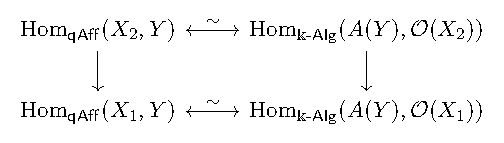
\includegraphics{lectures/5/pictures/cd_2.pdf}
	    \end{center}

	    И, если же у нас есть морфизм $Y_1 \to Y_2$, то мы получим коммутативную диаграмму:  
	    \begin{center}
	    	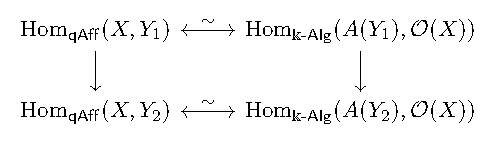
\includegraphics{lectures/5/pictures/cd_3.pdf}
	    \end{center}

	    \end{statement}

	    \begin{proof}
	    	Пусть задан морфизм $\varphi\colon X \to Y$, тогда он переводит регулярные функции на $Y$ в регулярные функции на $X$ (при помощи пуллбека). Значит, он индуцирует отображение $\varphi^*\colon \cO(Y) \to \cO(X)$:
	    	\[
	    		f \in \cO(Y), \quad f \mapsto \varphi^*(f) \in \cO(X).
	    	\]
	    	Совершенно ясно, что это отображение является гомоморфизмом $\bk$-алгебр. По теореме~\ref{O(X) = A(X)}, $\cO(Y) \cong A(Y)$, так что мы получаем гомомоифизм $A(Y) \to \cO(X)$. 

	    	Теперь построим обратное отображение. Пусть задан гомомомрфизм $\bk$-алгебр $h\colon A(Y) \to \cO(X)$. $Y$~--- аффинное, так что  $A(Y) = \bk[x_1, \ldots, x_n]/I(Y)$. Рассмотрим $\xi_i = h(\overline{x_i}) \in \cO(X)$, Эти функции определены на всём $X$, так что мы можем определить отображение 
	    	\[
	    		\psi\colon X \to \AA^n, \quad \psi(P) = (\xi_1(P), \ldots, \xi_n(P)).
	    	\]
	    	Покажем, что на самом деле $\psi$ действует в $Y$. Так как $Y = Z(I(Y))$,  достаточно показать, что $\forall f \in I(Y), \forall P \in X \ f(\psi(P)) = 0$. Так как $f$~--- многочлен, а $h$~--- гомоморфизм $\bk$-алгебр, 
	    	\[
	    	   	f(\psi(P)) = f((\xi_1(P), \ldots, \xi_n(P))) = h(f(\overline{x_1}, \ldots, \overline{x_n}))(P) = 0,
	    	   \]   
	    	так как $f \in I(Y)$. Так по гомоморфизму $\bk$-алгебр $h\colon A(Y) \to \cO(X)$ мы построили отображение $\psi\colon X \to Y$. То, что $\psi$~--- морфизм, напрямую вытекает из предложения~\ref{morph_criterion}.
	    \end{proof}
 
	    Заметим, что если оба многообразия аффинные, то мы получаем соответствие (естественный изоморфизм) 
	    \[
	    	\Hom_{\qAff}(X, Y) \xrightarrow{\sim} \Hom_{\Bbbk\text{-}\Alg}(A(Y), A(X)).
	    \]
	    То есть, мы получаем функтор $\qAff^{op}_{\Bbbk} \to \Bbbk\text{-}\Alg$ (где алгебры конечнопорожденные и редуцированные\footnote{Допуская вольность речи, мы обозначаем эти две категории одинаково и отличаем их в зависимости от контекста. }):
	    \[
	    	A\colon \qAff^{op}_{\Bbbk} \to \Bbbk\text{-}\Alg, \quad X \mapsto A(X).
	    \]
	    Кроме того, мы видели, что есть и обратный функтор: если $A \in \Bbbk\text{-}\Alg$, то мы можем рассмотреть аффинное многообразие $X'$ такое, что $A(X') \cong A$ и сопоставить $A \to X'$. Этот функтор задан корректно, так как если взять другое многообразие $X$ такое, что $A(X) \cong A(X')$, то изоморфизм алгебр будет индуцировать и изоморфизм многообразий $X \cong X'$ (так как функтор переводит изоморфизмы в изоморфизмы). 

	    Таким образом, мы доказали такую теоремы: 
	    \begin{theorem}\label{antieq_cat_1} 
	    	Категория квазиаффинных многообразий $\qAff$ антиэквивалентна категории конечнопорожденных редуцированных $\bk$-алгебр.  
	    \end{theorem}

     Переводя это на существенно менее изысканный язык, мы получаем такое следствие 

     \begin{corollary}
         Аффинные многообразия $X$ и $Y$ изоморфны тогда и только тогда, когда их аффинные координатные кольца $A(X)$ и $A(Y)$  изоморфны как $\bk$-алгебры. 
     \end{corollary}

	
	\subsection{Рациональные функции}


	\begin{definition}\label{rat_func}
		Пусть $X$~--- неприводимое аффинное многообразие, $U, V$~--- непустые открытые подмножества, а $f$ и $g$~--- регулярные функции на $U$ и $V$ соотвественно. Тогда будем говорить, что $(U, f) \sim (V, g)$ если $f = g$ на $U \cap V$.

		Класс эквивалентности по этому отношению мы будем называть \emph{рациональной функцией}.  

		\emph{Областью определения} рациональной функции называется объединение всех $U$ таких, что функция эквивалентна $(U, f)$ для некоторой $f$.
	\end{definition}

	\begin{remark}
		Множество всех рациональных функций на $X$ образует поле, которое мы будет обозначать через $\bk(X)$. 

		Проверим, что это в самом деле поле. Так как $X$ неприводимо, любые два непустых открытых подмножества $X$ имеют непустое пересечение (по~\ref{open_subset_of_irreducible}) и мы можем определить сложение и умножение, превратив $\bk(X)$ в кольцо. Кроме того, если $(U, f) \in K(X)$ и $f \neq 0$, то мы можем ограничить $f$ на открытое множество $V = U \setminus (U \cap Z(f))$, на котором $f$ не имеет нулей и тогда $1/f$ регулярна на $V$ и пара $(V, 1/f)$ будет обратным элементом к $(U, f)$. 
	\end{remark}

	Отметим, что для неприводимого аффинного многообразия $X$ определение поля рациональных функций $\Bbbk(X)$ можно дать несколько иначе от определения~\ref{rat_func}. 

	Предположем, что $X$ неприводимо, тогда мы можем рассмотреть поле частных координатного кольца $A(X)$. Кроме того, рассматривая очевидное отображение 
	\[
		A(X) \to \Bbbk(X).
	\]
	мы получаем и вложение поле $\mathrm{Frac}(A(X)) \hookrightarrow \Bbbk(X)$. С другой стороны, нетрудно видеть, что это изоморфизм. 





